\documentclass[aspectratio=43,t]{beamer}

% Colors
\usepackage{color}
\definecolor{mainorange}{HTML}{EC811B}
\definecolor{lightgrey}{HTML}{888888}

% Syntax highlighting
\usepackage{minted}
\usepackage{alltt}
\newcommand\hi[1]{{\color{mainorange} \textbf{#1}}}

% Theme
\usetheme[%
    sectionpage=none,
	subsectionpage=none,
	numbering=fraction,
	progressbar=foot,
]{metropolis}

% Customization
\setbeamertemplate{section in toc}[sections numbered]
\setbeamerfont{title}{size=\fontsize{30}{30}}
\setbeamerfont{block title}{size=\large}
\newcommand\sep{\textcolor{lightgrey}{\rule{\linewidth}{0.05mm}}}

% Meta
\title{LibrePCB}
\subtitle{A new, powerful and intuitive EDA tool for everyone}
\date{\today}
\author{Urban Bruhin}
\institute{}

\begin{document}

% ----------------------------------------------------------------- %

%\pgfdeclareimage[width=\paperwidth]{bg}{images/background-dark.pdf}
%\usebackgroundtemplate{\pgfuseimage{bg}}
\maketitle

% ----------------------------------------------------------------- %

%\begin{frame}[plain,noframenumbering]
%	\frametitle{Table of Contents}
%	\setcounter{tocdepth}{1}
%	\tableofcontents
%\end{frame}

% ----------------------------------------------------------------- %

%\pgfdeclareimage[width=\paperwidth]{bg}{images/background-light.pdf}
%\usebackgroundtemplate{\pgfuseimage{bg}}

\section{About LibrePCB}

\begin{frame}{\secname}
  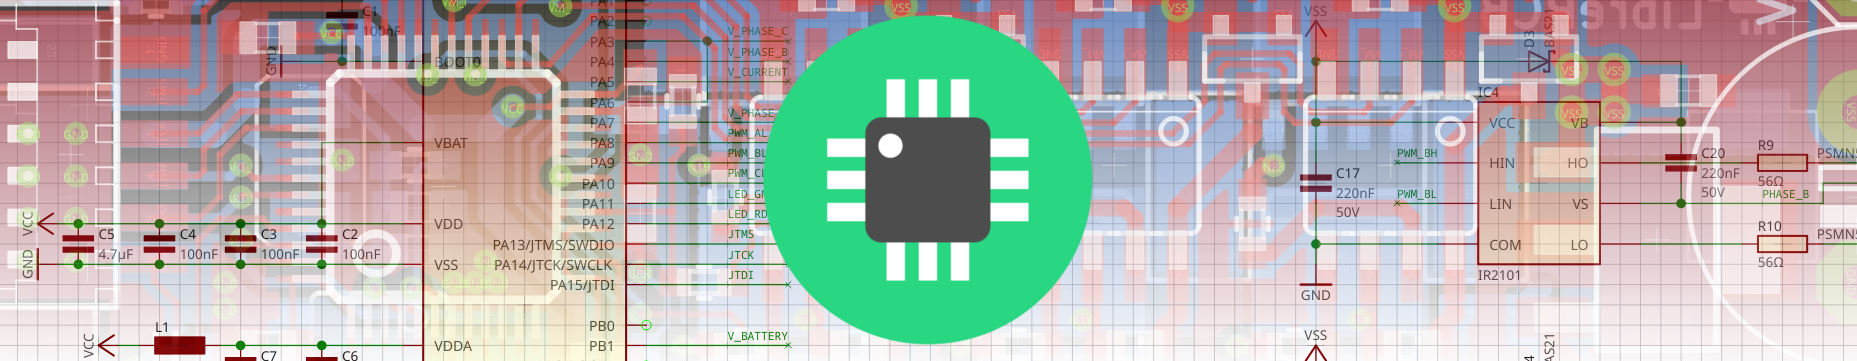
\includegraphics[width=\linewidth]{images/about_header.png} \linebreak\linebreak
  \textbf{Free/OpenSource EDA Suite}
  \begin{itemize}
    \item Multiplatform \faLinux\ \faApple\ \faWindows\
    \item Written from scratch in C++11/Qt5
    \item Development started in February 2013
    \item Website: \url{http://librepcb.org/}
    \item GitHub: \url{https://github.com/LibrePCB/LibrePCB}
  \end{itemize}
\end{frame}
\section{Contributing}

\begin{frame}{\secname}
  \begin{centering}
    \bigskip \bigskip
    \textbf{\Huge Contributors welcome!}\\
    \bigskip \bigskip
    {\footnotesize \url{https://github.com/LibrePCB/LibrePCB/blob/master/CONTRIBUTING.md}}\\
    {\footnotesize IRC: \texttt{\#librepcb} on Freenode}\\
  \end{centering}
  \textbf{\Large
    \begin{itemize}
      \centering
      \item Participate in issues
      \item Open pull requests
      \item Improve documentation
      \item Donate (Patreon, GitHub Sponsors, \dots)
    \end{itemize}
  }
\end{frame}


% ----------------------------------------------------------------- %

{
\setbeamertemplate{footline}{}
%\pgfdeclareimage[width=\paperwidth]{bg}{images/background-inverted.pdf}
%\usebackgroundtemplate{\pgfuseimage{bg}}
\begin{frame}[standout]
	\begin{centering}
	{\Huge Thank you!}\\
	{\normalsize \url{http://librepcb.org}}\\
	\end{centering}
\end{frame}
}

% ----------------------------------------------------------------- %

\end{document}
